\documentclass{beamer}

\newcommand{\delim}{\line(1,0){290}}
\newcommand{\norma}[1]{\Vert #1 \Vert_2}
\newcommand{\modulo}[1]{\vert #1 \vert}
\newcommand{\prodint}[2]{\langle #1,#2 \rangle}
\newcommand{\barrav}[1]{\line(0,1){#1}}
\newcommand{\ssiz}{\scriptsize}

\usepackage{multicol}

\colorlet{teal}[rgb]{green!50!blue}
%\setbeamercolor{cordotitulo}{bg=green!30!black,fg=white}
\useinnertheme{rounded}
\setbeamercolor{structure}{fg=teal!80!blue}
%\useoutertheme{smoothbars}
%\useoutertheme{shadow}
\useoutertheme[height=1 cm,width=1.5 cm]{sidebar}
%\usecolortheme{crane}
%\setbeamerfont{frametitle}{shape=\itshape}
\setbeamercolor{palette primary}{bg=teal!80!blue,fg=white}
\setbeamercolor{palette secondary}{bg=white,fg=white} %cor do logo
\setbeamercolor{palette tertiary}{bg=blue!70!black,fg=white}
\setbeamercolor{palette quaternary}{bg=white,fg=teal!80!blue}
\setbeamercolor{sidebar}{bg=teal!80!blue}
%\setbeamercolor{palette sidebar primary}{bg=red,fg=black}
%\setbeamercolor{palette sidebar secondary}{bg=red,fg=black}
\setbeamercolor{palette sidebar tertiary}{fg=white} %Autor no sidebar
\setbeamercolor{palette sidebar quaternary}{fg=white} %Titulo no sidebar
\setbeamercolor{section in sidebar}{fg=teal!80!blue,bg=white} %A cor naum
\setbeamercolor{subsection in sidebar}{fg=teal!80!blue,bg=white} %A cor naum
%ativa parece ser uma media das duas
%\setbeamercolor{section in sidebar current}{fg=red}
\setbeamercolor{frametitle}{fg=white,bg=teal!80!blue} %mudar
%fg aqui
\setbeamercolor{title}{bg=teal!80!blue,fg=white}
\setbeamerfont{title}{series=\bf}
\setbeamercolor{author}{bg=teal!80!blue,fg=white}
\setbeamerfont{author}{series=\bf}
\setbeamercolor{normal text}{bg=white,fg=teal!50!black}
\logo{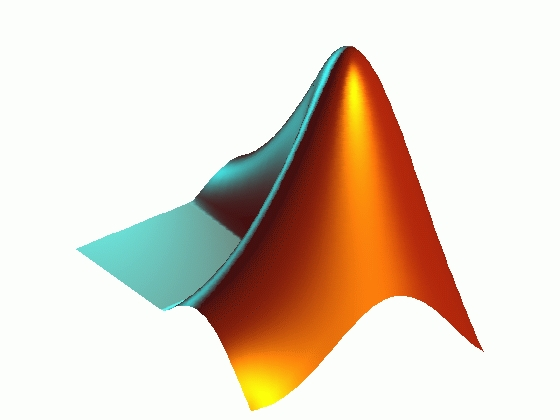
\includegraphics[scale=0.06]{matlab_logo.jpg}}

\title{Introdu\c{c}\~ao ao MatLab \\ Aula 5}
\author{Abel Siqueira \\ Kally Chung}
\date{}

\begin{document}

\frame{\titlepage}

\section[Gr\'aficos 2D]{}

\begin{frame}
\frametitle{Gr\'aficos 2D}

\begin{itemize}
 \item<1-> Uma das funcionalidades mais fortes do Matlab \'e gerar gr\'aficos.
 \item<2-> Este \'e o trunfo do Matlab sobre as outras linguagens.
 \item<3-> O Matlab gera gr\'aficos bidimensionais, gr\'aficos tridimensionais e curvas de n\'ivel, dentre outras possibilidades.
 \item<4-> Veremos primeiramente os gr\'aficos bidimensionais, gerados a partir de conjuntos de pontos, ou fun\c{c}\~oes.
\end{itemize}

\end{frame}
\subsection[Fun\c{c}\~ao plot]{}
\begin{frame}[fragile]
\frametitle{Fun\c{c}\~ao {\tt plot}}

\begin{itemize}
\item<1-> O comando {\tt plot} gera um gr\'afico utilizando dois conjuntos de
pontos, dentre outras op\c{c}\~oes.
\item<2-> O primeiro conjunto de pontos \'e respons\'avel pelos pontos no eixo
horizontal
\item<3-> O segundo conjunto de pontos \'e respons\'avel pelos valores
correspondentes no eixo vertical.
\item<4-> O comando conecta esses pontos por retas, na ordem em que foram
colocados no vetor.
\end{itemize}

\end{frame}

\begin{frame}[fragile]
\frametitle{Fun\c{c}\~ao {\tt plot}}

Exemplo 1:
{\scriptsize
\begin{verbatim}
>> x = [2 3 5 7]; y = [1 5 2 7];
>> plot(x,y)
\end{verbatim}}
\pause
Esse c\'odigo gera o gr\'afico
\begin{center}
\includegraphics[scale=0.3]{aula6ex1.jpg}
\end{center}
\pause
Note que os elementos de x est\~ao em ordem.
\end{frame}

\begin{frame}[fragile]
\frametitle{Fun\c{c}\~ao {\tt plot}}

Exemplo 2:
{\ssiz
\begin{verbatim}
>> x = [2 3 7 5]; y = [1 5 7 2];
>> plot(x,y)
\end{verbatim}
}
\pause
Esse c\'odigo gera o gr\'afico
\begin{center}
\includegraphics[scale=0.3]{aula6ex2.jpg}
\end{center}

\end{frame}

\begin{frame}[fragile]
\frametitle{Fun\c{c}\~ao {\tt plot}}

Tamb\'em conseguimos plotar aproxima\c{c}\~oes para fun\c{c}\~oes.
\pause

Exemplo 3:
{\ssiz
\begin{verbatim}
>> x = 2:0.01:4; y = sin(x);
>> plot(x,y)
\end{verbatim}
}
\pause
Esse c\'odigo gera o gr\'afico
\begin{center}
\includegraphics[scale=0.3]{aula6ex3.jpg}
\end{center}
\end{frame}

\begin{frame}[fragile]
\frametitle{Fun\c{c}\~ao {\tt plot}}

Outra maneira de gerar gr\'aficos para fun\c{c}\~oes \'e usar o {\tt for}.
\pause

Exemplo 4:
{\ssiz
\begin{verbatim}
>> x = -1:0.01:1; n = numel(x);
>> for i = 1:n
y(i) = sin(exp(-x(i)^2));
end
>> plot(x,y)
\end{verbatim}
}
\pause
Esse c\'odigo gera o gr\'afico
\begin{center}
\includegraphics[scale=0.3]{aula6ex4.jpg}
\end{center}
\end{frame}

\begin{frame}[fragile]
\frametitle{Fun\c{c}\~ao {\tt plot}}

O comando {\tt plot} tamb\'em permite plotar dois ou mais gr\'aficos juntos.
\pause

Exemplo 5:
{\ssiz
\begin{verbatim}
>> x = linspace(0,2,100); y = sin(x);
>> z = linspace(1,3,100); w = cos(z)+1;
>> plot(x,y,z,w)
\end{verbatim}}
\pause
Este c\'odigo gera o gr\'afico
\begin{center}
\includegraphics[scale=0.3]{aula6ex5.jpg}
\end{center}

\end{frame}

\begin{frame}[fragile]
\frametitle{Fun\c{c}\~ao {\tt plot}}

Tamb\'em podemos criar gr\'aficos com cores diferentes, marcadores nos pontos
dos dados e tipos de linhas diferentes.
\pause
Exemplo 6:
{\ssiz
\begin{verbatim}
>> x = linspace(0,2*pi,100); y = sin(x);
>> plot(x,y,`ro--')
\end{verbatim}
}
\pause
Esse c\'odigo gera o gr\'afico
\begin{center}
\includegraphics[scale=0.3]{aula6ex6.jpg}
\end{center}
\end{frame}

\begin{frame}[fragile]
\frametitle{Fun\c{c}\~ao {\tt plot}}

Os s\'imbolos para mudan\c{c}a de cores, marcadores e tipos de linha s\~ao:
{\tiny
\begin{center}
\begin{tabular}{|c|c|c|c|c|c|}
\hline
S\'imbolo & Cor & S\'imbolo & Marcador & S\'imbolo & Tipo de Linha \\ \hline
{\tt b} & Azul & . & Ponto & - & Linha Cont\'inua \\ \hline
{\tt g} & Verde & o & C\'irculo & : & Linha pontilhada \\ \hline
{\tt r} & Vermelho & x & Cruz & -. & Tra\c{c}os e Pontos \\ \hline
{\tt c} & Ciano & + & Sinal de Positivo & -- & Linha tracejada \\ \hline
{\tt m} & Magenta & * & Estrela ou Asterisco & & \\ \hline
{\tt y} & Amarelo & s & Quadrado & & \\ \hline
{\tt k} & Preto & d & Losango & & \\ \hline
{\tt w} & Branco & v & Tri\^angulo para baixo & & \\ \hline
& & \textasciicircum & Tri\^angulo para cima & & \\ \hline
& & $\langle$ & Tri\^angulo para esquerda & & \\ \hline
& & $\rangle$ & Tri\^angulo para direita & & \\ \hline
& & p & Pentagrama & & \\ \hline
& & h & Hexagrama & & \\ \hline
\end{tabular}
\end{center}
}

\end{frame}

\begin{frame}
\frametitle{Fun\c{c}\~ao {\tt plot}}

\begin{itemize}
 \item<1-> Podemos colocar linhas de grade no gr\'afico usando o comando {\tt
grid on}. Para retir\'a-las use {\tt grid off}.
 \item<2-> Para incluir nomes nos eixos horizontal e vertical utilize {\tt
xlabel(`nome')} e {\tt ylabel(`nome')} respectivamente.
 \item<3-> Para mudar o t\'itulo utilize {\tt title('titulo')}.
 \item<4-> Para mudar os limites horizontais e verticais do gr\'afico utilize
{\tt xlim(a,b)} e {\tt ylim(c,d)} respectivamente.
 \item<5-> Para mudar os dois simultaneamente utilize {\tt axis([a b c d])}.
 \item<6-> Para plotar mais gr\'aficos no gr\'afico j\'a existente, utilize o
comando {\tt hold on}. A partir da\'i, tudo que for desenhado aparecer\'a na
mesma janela.
\end{itemize}

\end{frame}

\begin{frame}[fragile]
 \frametitle{Fun\c{c}\~ao {\tt plot}}

Por exemplo:

\begin{multicols}{2}
{\ssiz
\begin{verbatim}
>> t = 0:0.05:10;
>> y = exp(-t.^2);
>> z = 1./(1+t.^2);
>> plot(t,y,'r')
>> grid on
>> title('Meu titulo')
>> xlabel('t')
>> ylabel('y')
>> hold on
>> plot(t,z,'k')
>> ylabel('y e z')
>> xlim([0 3]);
>> ylim([0 0.5]);
\end{verbatim}

\pause
Esses comandos geram o gr\'afico
\begin{center}
\includegraphics[scale=0.25]{aula6ex65.jpg}
\end{center}
}
\end{multicols}

\end{frame}


\begin{frame}
\frametitle{Fun\c{c}\~ao {\tt plot}}

\begin{itemize}
 \item<1-> Para abrir uma nova janela de gr\'afico utilize o comando {\tt
figure}.
 \item<2-> Para ativar a janela de n\'umero n, utilize {\tt
figure(n)}.
 \item<3-> Para fechar a janela ativa, use {\tt close}.
 \item<4-> O comando {\tt subplot(m,n,p)} divide a janela de gr\'afico em m por
n janelas, e ativa a subfigura de n\'umero p. A numera\c{c}\~ao \'e dada por
linhas, da esquerda para a direita.
 \item<5-> Daremos exemplo destes comandos posteriormente.
\end{itemize}

\end{frame}

\subsection[Fun\c{c}\~ao fplot]{}

\begin{frame}[fragile]
\frametitle{Fun\c{c}\~ao {\tt fplot}}

A fun\c{c}\~ao {\tt fplot} permite plotar fun\c{c}\~oes de uma maneira mais
r\'apida. Ela aceita arquivos m e function handle.
\pause
Exemplo 7:
{\ssiz
\begin{verbatim}
>> fplot(@exp,[0 1])
>> hold on
>> fplot(@(x) exp(x),[1,2],`r')
>> fplot(`exp',[2,3],`g')
>> xlim([0,3])
\end{verbatim}
}
\pause
Esse c\'odigo gera o seguinte gr\'afico
\begin{center}
\includegraphics[scale=0.3]{aula6ex7.jpg}
\end{center}

\end{frame}

\begin{frame}[fragile]
\frametitle{Fun\c{c}\~ao {\tt fplot}}

Podemos fazer coisas bem interessantes com o {\tt fplot}:
\pause

{\ssiz
\begin{verbatim}
>> f = @(x) exp(-10*x^2);
>> fplot(f,[-3,3]);
>> figure
>> g = @(x,t) f(x+t);
>> fplot(@(x) g(x,1),[-3,3]);
\end{verbatim}
Geramos os seguintes gr\'aficos:

\begin{center}
\includegraphics[scale=0.25]{aula6ex8a.jpg}
\includegraphics[scale=0.25]{aula6ex8b.jpg}
\end{center}

}

\end{frame}

\begin{frame}[fragile]
\frametitle{Fun\c{c}\~ao {\tt fplot}}

Continuando a partir dos comandos anteriores:

\begin{verbatim}
>> figure
>> N = 3; M = 4;
>> T = linspace(-3,3,M*N);
>> for i = 1:M
for j = 1:N
k = (i-1)*N+j;
subplot(M,N,k)
fplot(@(x) g(x,T(k)),[-10,10])
end
end
\end{verbatim}

\end{frame}

\begin{frame}
\frametitle{Fun\c{c}\~ao {\tt fplot}}

\begin{center}
Obtemos

\includegraphics[scale=0.4]{aula6ex9.jpg}
\end{center}

\end{frame}


\subsection[Outros Comandos]{}
\begin{frame}
\frametitle{Outros Comandos}
Al\'em dos comandos dados, ainda existem estes outros:
\begin{center}
\begin{tabular}{|c|c|}
\hline
Comando & Descri\c{c}\~ao \\ \hline
{\tt loglog} & Gr\'afico log-log \\ \hline
{\tt semilogx} & Gr\'afico semi-log no eixo x \\ \hline
{\tt semilogy} & Gr\'afico semi-log no eixo y \\ \hline
{\tt polar} & Gr\'afico em coordenadas polares \\ \hline
{\tt legend} & Acrescenta legenda. \\ \hline
{\tt text} & Coment\'ario acrescentado ao gr\'afico \\ \hline
{\tt area} & Hachura o gr\'afico \\ \hline
{\tt hist} & Histograma \\ \hline
{\tt errorbar} & Gr\'afico linear com barras de erro. \\ \hline
\end{tabular}
\end{center}
\end{frame}

\section[Exerc\'icios]{}

\begin{frame}
\frametitle{Exerc\'icios}

\begin{enumerate}
 \item Modifique a rotina do m\'etodo de newton de modo que ela guarde todas as itera\c{c}\~oes feitas. Tamb\'em modifique para que depois de encontrada a solu\c{c}\~ao, a rotina fa\c{c}a o gr\'afico da fun\c{c}\~ao e marque as itera\c{c}\~oes que o m\'etodo fez.
 \item Anteriormente programamos uma rotina que, dado $x_0$, verifica quantas itera\c{c}\~oes s\~ao necess\'arias para que apare\c{c}a o 1 na sequ\^encia
 \begin{eqnarray*}
 x_{k+1} = \left\{
 \begin{array}{ll}
 x_k/2 & \mbox {se $x_k$ \'e par,} \\
 3x_k+1 & \mbox {caso contr\'ario.}
 \end{array}
 \right.
 \end{eqnarray*}
 Fa\c{c}a uma rotina que recebe um elemento $N \in \mathbb{N}^{*}$ e que plota um gr\'afico com a quantidade de itera\c{c}\~oes para aparecer o 1 para todos os elementos entre 1 e $N$.
\end{enumerate}

\end{frame}

\begin{frame}
\frametitle{Exerc\'icios}
{\ssiz
\begin{enumerate}
\setcounter{enumi}{2}
 \item Lembre-se que na aula passada criamos
$$D_h[f](x) = \frac{f(x+h)-f(x)}{h} \approx f'(x).$$
Crie uma rotina que receba $f$, $f'$, $h$ e um intervalo $[a,b]$ e que fa\c{c}a o seguinte:
\begin{itemize}\ssiz
 \item Crie $D_h[f](x)$, usando Function Handle.
 \item Crie uma janela de figura, e a divida em duas.
 \item Na primeira delas, plote o gr\'afico de $D_h[f](x)$ em vermelho tracejado, e o gr\'afico de $f'(x)$ em preto cont\'inuo, no intervalo [a,b] utilizando {\tt fplot}.
 \item Plote o gr\'afico do erro entre $f'(x)$ e $D_h[f](x)$ para o $h$ e o intervalo dados, em verde pontilhado.
\end{itemize}
Teste com os seguintes dados:
\begin{itemize}\ssiz
 \item $f(x) = e^x, h = 0.5, [-1,2].$
 \item $f(x) = x^2-1, h = 0.1, [-1,1]$
 \item $f(x) = \sin(x), h = 0.25, [0, 2\pi]$
 \item $f(x) = \dfrac{x^2}{x^2+1}, h =0.1, [-1,1]$
\end{itemize}
\end{enumerate}
}

\end{frame}

\end{document}